\documentclass[]{scrartcl}
\usepackage[utf8]{inputenc}

\usepackage{placeins}
\usepackage[T1]{fontenc}
\usepackage[T2A]{fontenc}
\usepackage[finnish]{babel}
\usepackage{linguex} 
\usepackage{longtable} 
\usepackage{booktabs}
\usepackage{amsthm}
\usepackage{graphicx}
\newtheorem{maar}{Määritelmä}
\usepackage{fixltx2e} % provides \textsubscript
\usepackage{textcomp} % provides \textsubscript
\usepackage{hyperref}
\usepackage{xcolor}

\providecommand{\tightlist}{%
  \setlength{\itemsep}{0pt}\setlength{\parskip}{0pt}}

\hypersetup{
    colorlinks,
    linkcolor={red!50!black},
    citecolor={blue!50!black},
    urlcolor={blue!80!black}
}
\author{Juho Härme}
\title{Morfologia-kurssin luentomateriaaleja}
\date{\today}
\begin{document}
\maketitle
\tableofcontents
\newpage



\section{Luennot 12--13: persoona kieliopillisena kategoriana 2 ja
partisiippien
muodostus}\label{luennot-1213-persoona-kieliopillisena-kategoriana-2-ja-partisiippien-muodostus}

\begin{itemize}
\tightlist
\item
  \href{https://mustikka.uta.fi/~juho_harme/morfologia/\#tästä-kurssista}{Takaisin
  sivun ylälaitaan}
\item
  \href{http://mustikka.uta.fi/~juho_harme/morfologia/materiaalit/luento12.pdf}{Lataa
  PDF}
\item
  \href{http://mustikka.uta.fi/~juho_harme/morfologia/presentations/luento12.html}{Tutki
  luentokalvoja}
\item
  \href{http://mustikka.uta.fi/~juho_harme/morfologia/tehtavat/luento12.pdf}{Tutki
  tuntitehtäviä}
\end{itemize}

Jatketaan konjugaatioiden tutkimista. Tällä luennolla perehdytään
siihen, \emph{mistä voi tietää jonkin verbin kuuluvan ensimmäiseen tai
toiseen konjugaatioon} ja toisaalta siihen, minkälaisia verbejä jää
mainittujen kahden konjugaation ulkopuolelle.

\subsubsection{Milloin mikäkin
konjugaatio?}\label{milloin-mikuxe4kin-konjugaatio}

Ensimmäinen konjugaatio on venäjässä ylivoimaisesti toista yleisempi.
Asia on intutiivisestikin selvä, mutta katsotaan kokeeksi vähän
tilastoja wikisanakirjan datan avulla\footnote{Data on vapaasti
  käytettävissä ja ladattavissa
  \href{https://dumps.wikimedia.org/ruwiktionary}{täältä}.}.

Venäjän wikisanakirjan 5.10.2016 saatavilla olleessa versiossa on
listattuna\\
yhteensä 27307 verbiä. Näistä 22648 verbille on määritetty tai melko
helposti määriteltävissä\footnote{Muokkasin dataa siten, että mikäli
  tiedoista puuttui konjugaatio juuri tietylle verbille (esim.
  напариться) mutta konjugaatio löytyi verbin prefiksittömälle
  (johtamattomalle) versiolle (париться) tai postfiksittomalle
  versiolle, määriteltiin johdetun verbimuodon konjugaatioksi
  johtamattoman (tai postfiksittoman) verbin konjugaatio. Prosessi ei
  ole virheetön, mutta vähentää määrittelemättömien tapausten määrää
  merkittävästi. Tarkka kuvaus tehdystä analyysista saatavilla
  \href{https://github.com/hrmJ/morfologia/blob/master/wikianalysis.Rmd}{täältä}}
konjugaatio. Wikisanakirja käyttää verbitaivutuksen luokitteluun
Zaliznjakin monimutkaisempaa luokittelua, jossa on kaiken kaikkiaan 16
eri taivutusryhmää. Nämä on kuitenkin tässä kokeessa yhdistetty niin,
että vaihtoehtoina on ainoastaan ensimmäinen konjugaatio, toinen
konjugaatio tai poikkeuksellinen taivutus. Jos tarkastellaan verbejä,
joille Wikisanakirjassa on edellä kuvatulla tavalla määritettävissä
konjugaatio, voidaan eri konjugaatioiden yleisyyttä kuvata seuraavasti:

\FloatBarrier
\begin{figure}[htbp]
\centering
    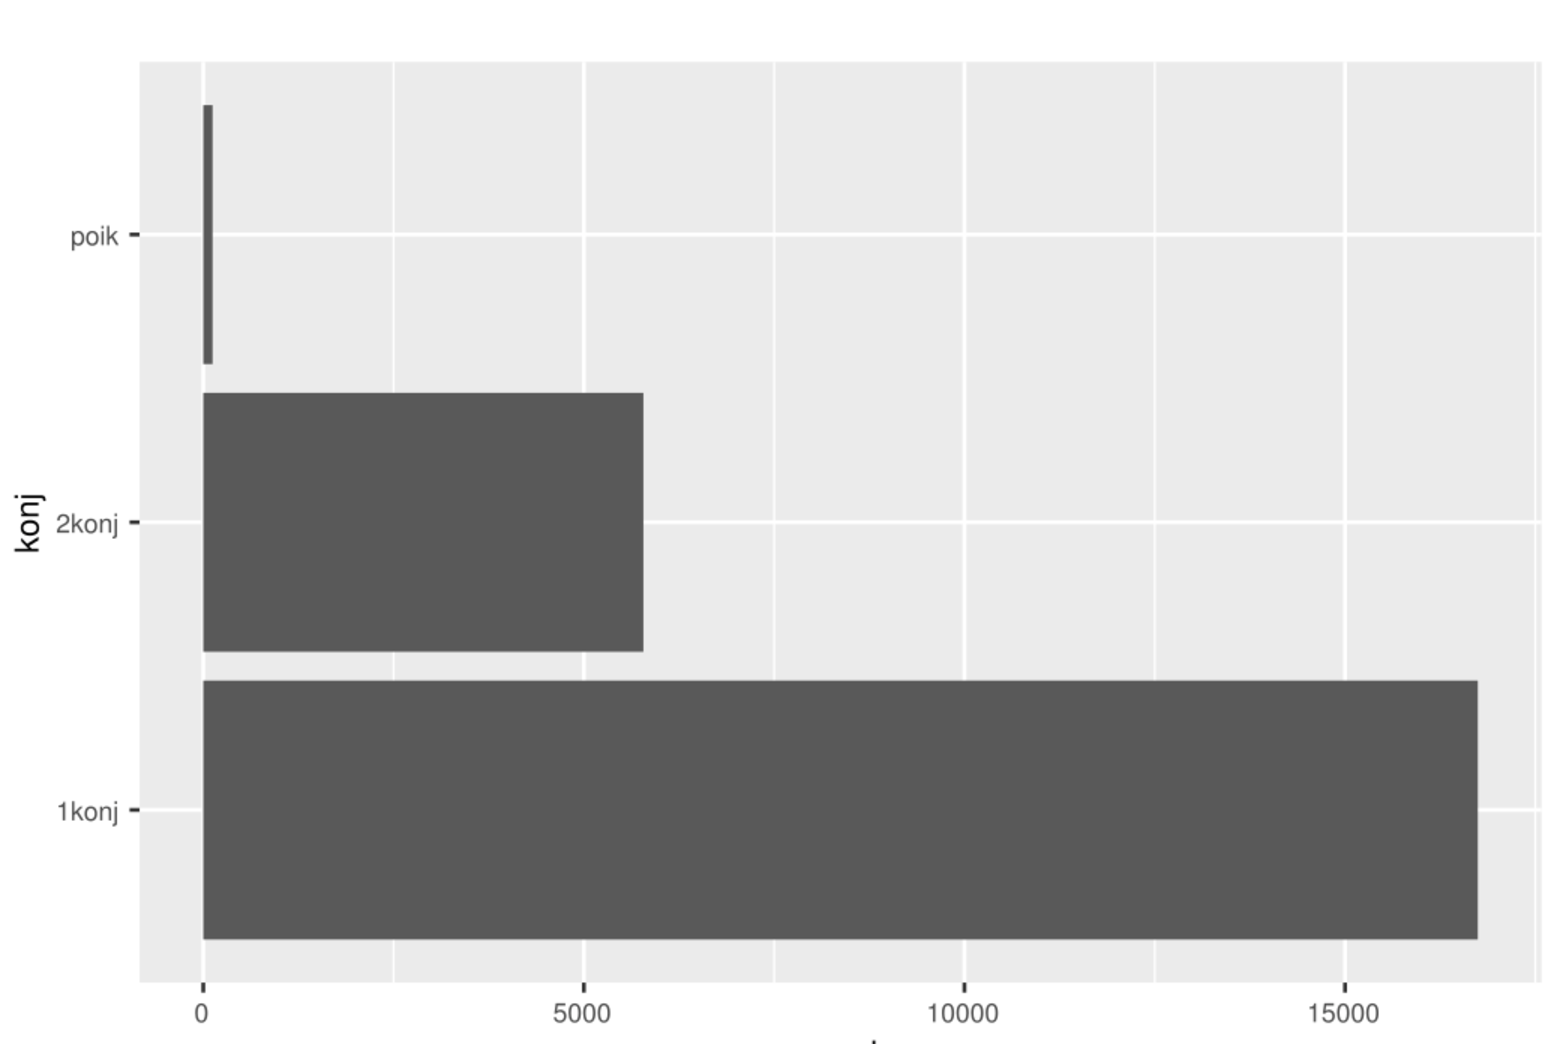
\includegraphics[width=0.9\textwidth,keepaspectratio]{../figure/wikidata.pdf}
\caption{Konjugaatioiden yleisyydet Wikisanakirjassa}
\end{figure}
\FloatBarrier

Kuvio osoittaa, että ensimmäiseen konjugaatioon kuuluvien verbien määrä
on huomattavan suuri verrattuna toisen konjugaation verbeihin: tarkkaan
ottaen 16744 verbiä siinä missä toiseen konjugaatioon voidaan laskea
5782 verbiä ja poikkeuksellisiin 122 verbiä. Tilastot eivät varmasti
poikkeusten osalta ole ehdottoman tarkkoja, mutta yhtä kaikki kokeilu
antaa hyvän vahvistuksen sille, että 1. konjugaation verbit todella ovat
selkeässä enemmistössä.

Koska toinen konjugaatio on huomattavasti harvinaisempi, se on hyvä
paikka aloittaa, kun yrittää miettiä, mistä minkäkin taivutustyypin
tunnistaa. Šeljakin (2006: 125--126) esittää, että infinitiivivartalon
perusteella voidaan päätellä verbi 2. konjugaatioon kuuluvaksi, jos

\begin{enumerate}
\def\labelenumi{\arabic{enumi}.}
\tightlist
\item
  infinitiivivartalo päättyy /и/-äänteeseen \emph{eikä ole osa
  juurimorfia}. Tästä seuraa, että verbit tyyppiä женить, учить,
  звонить, просить ovat toisen konjugaation verbejä, mutta verbit пить,
  шить, бить ensimmäisen, samoin kuin verbit брить (`ajaa (partaa)') ja
  гнить (`pilaantua'). Tämä on ylivoimaisesti suurin ryhmä:
  Wikisanakirjadatan 2. konjugaation sanoista peräti 5086 päättyy
  infinitiivissä \emph{ить}.
\item
  infinitiivivartalo päättyy /а/-vokaaliin, jota edeltää suhuäänne, eikä
  /а/-vokaali säily preesensvartalossa. Tämä tarkoittaa verbejä tyyppiä
  слышать, держать, прозвучать, лежать. Lisäksi a:han ilman suhuäännettä
  päättyvät спать ja гнать. Jos /a/ säilyy preesensvartalossa, kyseessä
  on 1. konjugaation sana (обещать ym.). Wikisanakirjan aineistossa
  tämän ryhmän sanoja on 243.
\item
  infinitiivivartalo päättyy /а/-vokaaliin ja sitä edeltää vokaali
  j-äänne: стоять, бояться. Wikisanakirjadatassa näitä tapauksia on 27
  ja kaikki ovat johdoksia edellä mainituista kahdesta verbistä
  (esimerkiksi простоять, достояться, побояться ym.)
\item
  infinitiivimuoto päättyy -еть, eikä е säily preesensvartalossa.
  Tällaisia sanoja on Wikisanakirja-aineistossa 373, esimerkiksi
  прозвенеть, оглядеть, смотреться, захрапеть ym -- usein kyseessä on
  jokin äänen lähettämiseen liittyvä verbi kuten храпеть, звенеть. Jos е
  säilyy preesensvartalossa, verbi kuuluu 1. konjugaatioon kuten
  esimerkiksi покраснеть.
\end{enumerate}

\subsection{Infinitiivi- ja preesensvartaloiden suhteista ensimmäisessä
deklinaatiossa}\label{infinitiivi--ja-preesensvartaloiden-suhteista-ensimmuxe4isessuxe4-deklinaatiossa}

Tarkastellaan vielä ensimmäisen deklinaation tärkeimpiä sisäisiä
sanaryhmiä, joita tässä erotellaan seitsemän.

\subsubsection{1. ryhmä}\label{ryhmuxe4}

Produktiivisin ja ylivoimaisesti suurin ryhmä ovat verbit tyyppiä
\emph{читать}, joissa infinitiivivartalon lopussa on jokin vokaaleista
а, е, и/ы tai у (Шелякин 2006: 127). Yhteistä tälle ryhmälle on, että
preesensvartalo loppuu /j/-äänteeseen: читать - читаj-, покраснеть -
покраснеj, дуть - дуj. Tämän lisäksi infinitiivivartalon viimeinen
vokaali on preesensvartalossa joskus eri: открыть - откроj, мыть - моj,
брить - брej sekä и--j-vaihtelu sanoissa ltyyppiä /бить/--/бью/т
(foneettisesti: /би/т'/--/бj/ут/).

\subsubsection{2. ryhmä}\label{ryhmuxe4-1}

Toisen 1. konjugaation sisäisen ryhmän muodostavat ne tutut verbit,
joiden infinitiivivartalo päättyy /ова/ (tai /ева/) ja preesensvartalo
/уj/: /интрес/ова/ -- /интерес/уj/, /жева/ -- /жуj/ (жевать, `purra').

\subsubsection{3. ryhmä}\label{ryhmuxe4-2}

Hieman edellisen kaltainen ryhmä ovat verbit tyyppiä давать. Näillä
infinitiivivartalon loppu on muotoa /ава/ ja preesensvartalo /аj/.
Ryhmään kuuluvat esimerkiksi /признава/ть/ -- /призна/j/, /устава/ть/ --
/устаj/.

\subsubsection{4. ryhmä}\label{ryhmuxe4-3}

Seuraavaksi ryhmäksi voidaan erottaa verbit tyyppiä \emph{писать}.
Näissä infinitiivivartalo päättyy /а/-vokaaliin, ja preesensvartalo
eroaa infinitiivivartalosta juurimorfin viimeisen konsonantin osalta:
/писа/ -- /пиш/, /плака/ -- /плач/.\footnote{Huomaa, ettei näitä verbejä
  pidä sekoittaa niihin ensimmäisen konjugaation verbeihin, joilla
  tapahtuu preesensvartalon sisällä äänteenmuutos /о/-alkuisissa
  muodoissa (ks. жить edellä).} Šeljakinin (2006: 129) mukaan tämän
tyypin verbejä on noin sata (писать, сказать, двигать,
махать,искать,брызгать ym.).

\subsubsection{5. ryhmä}\label{ryhmuxe4-4}

Verbit, joiden infinitiivivartalo päättyy \emph{ну}, voidaan jakaa
kahteen ryhmään sen perusteella, miten niiden preteritimuodot
muodostetaan. Ensimmäiseen ryhmään kuuluvat \emph{momentaaniset}
(одноактный) verbit tyyppiä толкнуть, joilla preteritimuoto muodostetaan
suoraan infinitiivivartalon perusteella (/толкну/л/). Toisen ryhmän
muodostavat verbit tyyppiä \emph{остынуть} (`jäähtyä, haaleta'), jotka
ilmaisevat astettaista olotilan muutosta ja joiden preteritimuodoissa
ну-suffiksi katoaa taivutuspäätteen edeltä (остыл). Näitä jälkimmäisiä
verbejä on selvästi vähemmän, Šeljakinin (2006: 129) mukaan noin
viisikymmentä. Kummassakin tapauksessa preesensvartalo päättyy /н/
(толкн -- остын). Yhteensä näitä ryhmiä edustaa Wikisanakirjan
aineistossa 926 verbiä, esimerkiksi подвинуть, шагнуть, замёрзнуть
(preteriti замёрз).

\subsubsection{6. ryhmä}\label{ryhmuxe4-5}

Šeljakin (2006: 133) laskee perustellusti omaksi ryhmäkseen verbit
tyyppiä начать/обнять (`halata') / понять/нажать (`painaa'), joissa
preesensvartalo eroaa melko selkeästi infinitiivivartalosta. Muodostus
noudattaa mallia /нача/ -- /начн/, /обня/ -- /обним/, /поня/ -- /пойм/,
/нажа/ -- /нажм/. Kaikissa tapauksissa siis preesensvartaloon ilmestyy
nasaali /м/ tai /н/ sekä tämän lisäksi joko /и/ tai /j/.

\subsubsection{7. ryhmä}\label{ryhmuxe4-6}

Ehkä haastavimman ryhmän muodostavat verbit, joissa tapahtuu edellä
mainittu äänteenmuutos muissa kuin yksikön ensimmäisessä ja monikon
kolmannessa persoonassa. Lisäksi tämän ryhmän verbeillä esiintyy
esimerkiksi väistyvän vokaalin ilmiötä. Ryhmän muodostavat seuraavat
alaluokat:

\begin{itemize}
\tightlist
\item
  infinitiivissä \emph{-чь} päättyvät verbit tyyppiä печь, жечь, лечь,
  joilla infinitiivi- ja preesensvartalot ovat identtiset. Huomaa
  väistyvä vokaali жечь-verbillä (infinitiivi жечь, mutta preesensmuodot
  /жг/у, /жжёшь/ jne.) лечь-verbillä puolestaan on preesensmuodoissa
  vartalon lopussa a-vokaali: лягу, ляжешь ym.
\item
  infinitiivissä /сти/ tai /зти/ tai /сть/ päättyvät verbit kuten
  нести,спасти, везти, красть ja попасть. Näillä verbeillä äänteenmuutos
  tapahtuu liudentumattomien ja liudentuneiden konsonanttien välillä,
  kuten (selvyyden vuoksi foneettisesti esitettynä) /вез/у -- /вез'/ош
  ja /попад/у -- /попад'/ош/. Osalla сти-infinitiivin saavista verbeistä
  sekä kaikilla сть-infinitiivin saavista preteritin vartalo päättyy
  vokaaliin ja saa peräänsä normaalin л-tunnuksen (vrt. везти -- вёз ja
  брести -- брёл / попасть -- попал).
\item
  Edellisen kaltainen alaryhmänsä ovat verbit плыть ja жить, joilla
  preesensvartalo loppuu infinitiivivartalossa esiintymättömään
  в-konsonanttiin ja on siis muotoa /жив/ tai /плыв/ ja joilla myös
  toteutuu äänteenmuutos liudentuneiden ja liudentumattomien
  konsonanttien välillä. Vastaavasti verbillä учесть preesensvartalossa
  on ``ylimääräinen'' \emph{т}: учесть -- /учт/. Myös verbit tyyppiä
  умереть kuuluvat tähän ryhmään: niilläkin tapahtuu vaihtelu
  liudentuneen ja liudentumattoman konsonantin välillä. Lisäksi
  havaitaan väistyvä vokaali: infinitiivivartalo on muotoa /умере/,
  preesensvartalo /умр/.
\end{itemize}

\subsection{Epäsäännöllisesti taipuvia
verbejä}\label{epuxe4suxe4uxe4nnuxf6llisesti-taipuvia-verbejuxe4}

Edellä käsiteltiin etenkin ensimmäiseen konjugaatioon liittyviä paikoin
melko monimutkaisiakin eroja infinitiivi- ja preesensvartaloiden välillä
sekä preesensvartalon sisällä tapahtuvia äänteenmuutoksia niin
ensimmäisessä kuin toisessakin konjugaatiossa. Vaikka kuvatut ilmiöt
tekevät venäjän verbitaivutuksesta melko laajan ilmiön, voidaan todeta,
että loppujen lopuksi suuri osa verbeistä sopii kuitenkin joko
ensimmäiseen tai toiseen konjugaatioon -- poikkeuksia ja
sekataivutustapauksia ei ole älyttömän paljon. Wikisanakirjan
aineistossa varsinaisten poikkeustapausten luokkaan osuu vain 122
tapausta (mukana paljon johdoksia) kaikkiaan noin 27 000
verbilekseemistä . Merkittävimpiä näistä lienevät
\href{http://ru.wiktionary.org/wiki/хотеть}{хотеть},
\href{http://ru.wiktionary.org/wiki/бежать}{бежать},
\href{http://ru.wiktionary.org/wiki/дасть}{дасть} ja
\href{http://ru.wiktionary.org/wiki/есть}{есть} (linkit
Wikisanakirjaan). Kaksi ensimmäistä sekoittavat 1. ja 2. deklinaation,
дать-verbissä on tyystin omat päätteensä ja есть-verbilläkin yksikön
ensimmäinen persoona saa aivan oman, muista slaavilaisista kielistä
kuten tsekistä tutun m-päätteen sekä eräitä muutoksia preesensvartaloon.

\subsection{Muutama sana painoista}\label{muutama-sana-painoista}

Tässä yhteydessä verbien painotyyppeihin ei perehdytä yhtä tarkasti kuin
substantiivien. Šeljakinin (2006: 136) perusteella voidaan kuitenkin
todeta, että verbit jakautuvat painon puolesta kolmeen pääryhmään:

\begin{enumerate}
\def\labelenumi{\arabic{enumi}.}
\tightlist
\item
  Paino aina vartalolla

  \begin{itemize}
  \tightlist
  \item
    Tähän kuuluvat kaikki verbit, joiden infinitiivi päätty painottomaan
    \emph{ать}-tavuun kuten
    \href{http://ru.wiktionary.org/wiki/обЕдать}{обЕдать},
    \href{http://ru.wiktionary.org/wiki/лАять}{лАять},
    \href{http://ru.wiktionary.org/wiki/Ехать}{Ехать} ym. Muutenkin
    edellä esitetty 1. konjugaation ensimmäinen ja suurin alaryhmä
    sisältää käytännössä vain tähän painotyyppiin kuuluvia verbejä
    (poikkeuksena verbit tyyppiä
    \href{http://ru.wiktionary.org/wiki/бить}{бить} /
    \href{http://ru.wiktionary.org/wiki/петь}{петь}). Lisäksi suurin osa
    \emph{ова/ева}-suffiksillisista verbeistä (toinen 1. konjugaation
    alaryhmä) kuuluu tähän ryhmään.
  \end{itemize}
\item
  Paino aina päätteellä

  \begin{itemize}
  \tightlist
  \item
    Tähän päätetyyppiin kuuluu suurin osa edellä 1. konjugaation
    seitsemänneksi alaryhmäksi luokitelluista verbeistä
    (\href{http://ru.wiktionary.org/wiki/жить}{жить},
    \href{http://ru.wiktionary.org/wiki/нести}{нести},
    \href{http://ru.wiktionary.org/wiki/красть}{красть} ym. MUTTA
    \href{http://ru.wiktionary.org/wiki/лечь}{лечь},
    \href{http://ru.wiktionary.org/wiki/сесть}{сесть}). Toinen suuri
    tyhmä ovat toisen konjugaation verbit, joiden infinitiivi loppuu
    painolliseen
    /ить/-tavuun(\href{http://ru.wiktionary.org/wiki/звонить}{звонить},
    \href{http://ru.wiktionary.org/wiki/творить}{творить} ym.). Lisäksi
    joitakin ова/ева-verbejä
    (\href{http://ru.wiktionary.org/wiki/жевать}{жевать},
    \href{http://ru.wiktionary.org/wiki/основать}{основать},
    \href{http://ru.wiktionary.org/wiki/клевать}{клевать} ym.) ja kaikki
    ава-verbit (\href{http://ru.wiktionary.org/wiki/давать}{давать},
    \href{http://ru.wiktionary.org/wiki/признать}{признать} ym.).
  \end{itemize}
\item
  Paino aina vartalolla paitsi yksikön ensimmäisessä persoonassa

  \begin{itemize}
  \tightlist
  \item
    Tähän päätetyyppiin kuuluvat kaikki edellä neljänneksi 1.
    konjugaation alaryhmäksi luetellut verbit, jos ne loppuvat
    infinitiivissä painolliseen \emph{ать}-tavuun (писать, махать).
    Lisäksi tähän kuuluu parikymmentä 2. konjugaation painolliseen
    \emph{ить}-tavuun infinitiivissä päättyvä verbiä kuten
    \href{http://ru.wiktionary.org/wiki/водить}{водить},
    \href{http://ru.wiktionary.org/wiki/купить}{купить} ja
    \href{http://ru.wiktionary.org/wiki/ловить}{ловить}.
  \end{itemize}
\end{enumerate}

\subsection{Partisiippien muodostus}\label{partisiippien-muodostus}

Pohjustetaan nyt tulevaa luentoa pääluokista käymällä läpi vielä yhtä
sananmuodostusoppiin liittyvää teemaa: partisiippien muodostusta.

\subsubsection{Mitä partisiipit ovat?}\label{mituxe4-partisiipit-ovat}

Verbeillä on niin suomessa kuin venäjässä kahdenlaisia muotoja:
persoonamuotoja (спрягаемые формы глагола) ja nominaali- eli
infiniittimuotoja (неспрягаемые формы глагола). Persoonamuodot taipuvat
suomalaisen nimityksensä mukaisesti persoonissa tai venäjän tapauksessa
menneen ajan muotojen osalta suvussa ja luvussa. Nominaalimuodot
puolestaan muistuttavat taivutukseltaan ja osin myös syntaktiselta
käyttäytymiseltään nomineja, esimerkiksi adjektiiveja. Partisiipit ovat
nominaalimuoto, joita on sekä suomessa että venäjässä mutta jotka eivät
kuitenkaan näissä kahdessa kielessä muodosta identtisiä kategorioita.

Venäjässä partisiipit voidaan jakaa neljään ryhmään riippuen niiden
edustamasta \emph{aikamuodosta} ja \emph{pääluokasta} (molemmat verbien
ilmaisemia kieliopillisia kategorioita).

\begin{enumerate}
\def\labelenumi{\arabic{enumi}.}
\tightlist
\item
  Aktiivin partisiipit

  \begin{itemize}
  \tightlist
  \item
    aktiivin partisiipin preesensmuoto ilmaisee jonkin subjektin jotakin
    ominaisuutta nykyhetkessä: человек, \emph{несущий} ящик. Suomessa
    tätä vastaa niin kutsuttu VA-partisiippi (ks.
    \href{http://scripta.kotus.fi/visk/sisallys.php?p=521}{VISK §521}):
    laatikkoa \emph{kantava} henkilö.
  \item
    aktiivin partisiipin preteritimuotoa puolestaan vastaa suomen
    NUT-partisiippi ja se ilmaisee vastaavaa ominaisuutta menneessä
    ajassa: человек, \emph{нёсший} ящик (laatikkoa \emph{kantanut}
    henkilö)
  \end{itemize}
\item
  Passiivin partisiipit

  \begin{itemize}
  \tightlist
  \item
    passiivin partisiipin preesensmuoto ilmaisee jonkun agentin jollekin
    kohteelle suorittamaa tai suoritettavissa olevaa toimintaa: ящик,
    несомый человеком (ihmisen kantama laatikko). Tätä vastaa usein
    suomen agenttipartisiippi mutta toisaalta, jos agenttia ei ilmaista,
    myös suomen VA-partisiipin passiivimuoto: vrt. \emph{допустимый} /
    \emph{hyväksyttävä}.
  \item
    passiivin partisiipin preteriti ilmaisee menneisyydessä suoritetun
    toiminnan ja mahdollisesti toiminnan suorittaneen agentin. Sitä
    vastaa suomen suomen TU-partisiippi: унесённый -- (pois) kannettu.
  \end{itemize}
\end{enumerate}

\subsubsection{Miten partisiipit
muodostetaan?}\label{miten-partisiipit-muodostetaan}

\paragraph{Rajoituksia}\label{rajoituksia}

Venäjän partisiipeissa on syytä kiinnittää huomiota siihen, ettei
kaikkia partisiippeja voi muodostaa kaikista verbeistä. Tarkastellaan
ensin, mitä puhtaan sananmuodostuksellisia rajoituksia partisiippien
muodostamiseen liittyy.

\subparagraph{Sananmuodostukselliset
rajoitukset}\label{sananmuodostukselliset-rajoitukset}

Pääpiirteissään sananmuodostuksen tasolla ovat voimassa seuraavat
rajoitukset:

\begin{enumerate}
\def\labelenumi{\arabic{enumi}.}
\tightlist
\item
  Niin aktiivin kuin passiivin partisiipin \textbf{preesensmuotoja}
  muodostetaan vain imperfektiivisen aspektin verbeistä.
\item
  \textbf{Passiivin partisiipin preteritimuotoja} muodostetaan vain
  perfektiivisen aspektin verbeistä.
\item
  \textbf{Aktiivin partisiipin preteritimuotoja} voidaan muodostaa
  aspektista riippumatta.
\end{enumerate}

\subparagraph{Käyttöön liittyvät
rajoitukset}\label{kuxe4yttuxf6uxf6n-liittyvuxe4t-rajoitukset}

Vaikka jokin partisiippimuoto voitaisiin teoriassa muodostaa, on usein
käytännössä niin, ettei muotoa kuitenkaan ole olemassa. Ensinnäkin
partisiippien käyttöä rajoittaa se syntaktinen seikka, että passiivin
partisiippimuotoja muodostetaan pääasiassa transitiiviverbeistä eli
verbeistä, jotka saavat täydennyksekseen suoran objektin (poikkeuksena
esimerkiksi руководить чем, josta voidaan muodostaa passiivin
partisiipin preesensmuoto). Šeljakin (2006: 177) huomauttaa lisäksi
erityisesti passiivin partisiipin preesensmuodoista, että ne ovat
tyyliltään kirjallisia, mistä johtuen monista arkipäiväisistä verbeistä
niitä ei todellisuudessa muodosteta: esimerkiksi verbeistä ругать,
кормить, крыть. Wade (2010: 369) antaa tarkemman luettelon siitä,
minkätyyppisistä verbeistä ei passiivin partisiipin preesensiä
muodosteta. Waden huomiot ovat pääpiirteissään seuraavia:

\begin{itemize}
\tightlist
\item
  Passiivin partisiipin preesensiä ei muodosteta verbeistä, joiden
  infinitiivi päättyy -чь, -уть, -ереть, -зть, -сть
\item
  Ei myöskään monista yksitavuisista verbeistä kuten бить, брать, мыть,
  шить
\item
  Ei useimmista edellä 1. konjugaation 4. alaryhmäksi nimitetyistä
  verbeistä (писать, плакать, прятать)
\item
  Monet 2. konjugaation verbit ovat sellaisia, ettei niistä muodosteta
  passiivin partisiipin preesensiä. Wade mainitsee esimerkkeinä mm.
  verbit благодарить, платить, портить ja чистить.
\end{itemize}

\paragraph{Vartalot}\label{vartalot}

Partisiipit muodostetaan venäjässä suffiksien avulla. Nikunlassin (2002:
163) mukaan muodostus voidaan (hieman yksinkertaistaen) tiivistää
toteamalla, että preesensmuotojen pohjana on preesensvartalo,
preteritimuotojen pohjana infinitiivivartalo. Näin ollen edellä
esimerkkinä toimineesta нести-verbistä voidaan preesensmuotojen osalta
todeta:

\begin{enumerate}
\def\labelenumi{\alph{enumi})}
\tightlist
\item
  Aktiivin partisiipin preesens:

  \begin{enumerate}
  \def\labelenumii{\arabic{enumii}.}
  \tightlist
  \item
    Preesensvartalo muodostetaan нести -- /нес/ут/ -- /нес/
  \item
    Aktiivin partisiipin preesens muodostetaan /ущ/-suffiksilla
  \item
    Aktiivin partisiipin preesensmuodon vartaloksi saadan /нес/ущ/
  \item
    Partisiippimuotojen taivutuspäätteet ovat adjektiivideklinaation
    mukaiset, joten aktiivin partisiipin preesensmuotoja нести-sanasta
    ovat /нес/у/щий/, /нес/ущ/ая/ ym.
  \end{enumerate}
\item
  Passiivin partisiipin preesens:

  \begin{enumerate}
  \def\labelenumii{\arabic{enumii}.}
  \tightlist
  \item
    Preesensvartalo muodostetaan нести -- /нес/ут/ -- /нес/
  \item
    Aktiivin partisiipin preesens muodostetaan /ом/-suffiksilla
  \item
    Aktiivin partisiipin preesensmuodon vartaloksi saadan /нес/ом/
  \item
    Partisiippimuotojen taivutuspäätteet ovat adjektiivideklinaation
    mukaiset, joten aktiivin partisiipin preesensmuotoja нести-sanasta
    ovat /нес/ом/ый/, /нес/ом/ая/ ym.
  \end{enumerate}
\end{enumerate}

Preteritimuotojen kohdalla on parempi käyttää esimerkkinä jotakin
säännöllisen infinitiivivartalon verbiä, esimerkiksi прочитать:

\begin{enumerate}
\def\labelenumi{\alph{enumi})}
\tightlist
\item
  Aktiivin partisiipin preteriti:

  \begin{enumerate}
  \def\labelenumii{\arabic{enumii}.}
  \tightlist
  \item
    Infinitiivivartalo muodostetaan /прочита/ть -- /прочита/
  \item
    Aktiivin partisiipin preteriti muodostetaan /вш/-suffiksilla
  \item
    Aktiivin partisiipin preteritimuodon vartaloksi saadaan /прочита/вш/
  \item
    Partisiippimuotojen taivutuspäätteet ovat adjektiivideklinaation
    mukaiset, joten aktiivin partisiipin preesensmuotoja
    прочитать-sanasta ovat /прочита/вш/ий, /прочита/вш/ая ym.
  \end{enumerate}
\item
  Passiivin partisiipin preteriti:

  \begin{enumerate}
  \def\labelenumii{\arabic{enumii}.}
  \tightlist
  \item
    Infinitiivivartalo muodostetaan /прочита/ть -- /прочита/
  \item
    Passiivin partisiipin preteriti muodostetaan /нн/-suffiksilla
  \item
    Aktiivin partisiipin preteritimuodon vartaloksi saadaan /прочита/нн/
  \item
    Partisiippimuotojen taivutuspäätteet ovat adjektiivideklinaation
    mukaiset, joten aktiivin partisiipin preesensmuotoja
    прочитать-sanasta ovat /прочита/нн/ый, /прочита/нн/ая ym. Lisäksi
    voidaan muodostaa lyhyet muodot /прочита/н/ø/,/прочита/н/а/ ym.,
    joissa /онн/-suffiksin sijasta on suffiksi /он/
  \end{enumerate}
\end{enumerate}

\paragraph{Suffiksit}\label{suffiksit}

Partisiippien muodostamisessa käytettävät suffiksit vaihtelevat jonkin
verran. Seuraavassa käydään läpi vaihtelut muodostussuffikseissa
partisiipeittain (tarkemmin ks. Nikunlassi 2002: 162, Шелякин (2006):
175--178).

\subparagraph{Preesenspartisiipit}\label{preesenspartisiipit}

Partisiippien preesensmuotojen muodostus on selkeää. Aktiivin
partisiipin preesensin suffikseja on kaksi: /ущ/ ja /ащ/. Nämä
jakautuvat siististi niin, että 1. konjugaation verbeillä suffiksi on
/ущ/, 2. konjugaation verbeillä /ащ/. Passiivin partisiipin
preesensmuodoissa 1. konjugaation suffiksi on /ом/ ja 2. konjugaation
suffiksi /им/. Huomaa jälleen kerran, että /ом/-suffiksin vokaali on
painollisen tavun jälkeinen redusoitunut /о/, jota liudentuneen
konsonantin tai j-äänteen jäljessä merkitään е-kirjaimella.

Tarkastellaan esimerkkiä kummastakin konjugaatiosta.

\begin{enumerate}
\def\labelenumi{\alph{enumi})}
\tightlist
\item
  Verbi /покупать/ kuuluu 1. konjugaatioon. Preesenspartisiipit
  muodostetaan preesensvartalosta, joka tässä tapauksessa on /покупаj/.

  \begin{itemize}
  \tightlist
  \item
    Aktiivin partisiipin tunnus 1. konjugaatiolla on /ущ/, joten
    muodoksi saadaan: /покупаj/ущ/ий/.
  \item
    Passiivin partisiipin tunnus 1. konjugaatiolla on /ом/ joten
    muodoksi saadaan /покупа/ем/ый (foneettisessa asussaan
    /покупаj/ом/ый)
  \end{itemize}
\item
  Verbi /держать/ kuuluu 2. konjugaatioon. Preesenspartisiipit
  muodostetaan preesensvartalosta, joka tässä tapauksessa on /держ/.

  \begin{itemize}
  \tightlist
  \item
    Aktiivin partisiipin tunnus 2. konjugaatiolla on /ащ/, joten
    muodoksi saadaan: /держ/ащ/ий/.
  \item
    Passiivin partisiipin tunnus 1. konjugaatiolla on /им/ joten
    muodoksi saadaan /держ/им/ый
  \end{itemize}
\end{enumerate}

Kuten todettu, preesenspartisiipit muodostetaan säännönmukaisesti
preesensvartalosta. Poikkeuksen muodostavat kuitenkin edellä 1.
konjugaation toiseksi alaryhmäksi nimetty joukko, jonka verbeillä
\emph{passiivin partisiipin} muodostus tapahtuu infinitiivivartalon
perusteella. Esimerkiksi sanat признавать ja давать saavat siis
muodoiksi признаваемый/даваемый (eivätkä preesensvartaloon pohjautuvia
*признаюемый/*даюемый).

\subparagraph{Aktiivin partisiipin
preteriti}\label{aktiivin-partisiipin-preteriti}

Aktiivin partisiipin preteritissä on myös kaksi eri vaihtoehtoa
suffiksille: /вш/ tai /ш/. Ensimmäistä käytetään, jos verbin
infinitiivivartalo päättyy vokaaliin, toista muussa tapauksissa.
Selkeitä sanoja tässä suhteessa ovat sanat, joilla infinitiivin tunnus
on tavallinen \emph{ть}: /прочита/вш/ий/, /игра/вш/ий,
/рассматрива/вш/ий jne. Enemmän pohdiskelua vaativat чь-, сть ja
сти-infinitiivit.

Pohditaan ensin чь-päätteisiä verbejä, esimerkiksi verbejä печь ja
стричь (`leikata hiuksia'). Edellä todettiin, että infinitiivivartalo on
näillä verbeillä preesensvartalon kaltainen eli muodostetaan /печь/ --
/пек/ут/ -- /пек/ ja /стричь/ -- /стриг/ут/ -- /стриг/. Näissä
tapauksissa infinitiivivartaloita ovat siis пек ja стриг, jotka
päättyvät konsonanttiin. Partisiipin muodostava suffiksi on siis /ш/,
joten aktiivin partisiipin preteritimuodot ovat /пёк/ш/ий/ ja
/стриг/ш/ий/ (huomaa kuitenkin painollinen о-vokaali пёкший-sanassa).

Myös сти-verbeistä todettiin edellä, että infinitiivivartalo on
preesensvartalon kaltainen. Näin ollen нести-verbin infinitiivivartalo
on /нести/ -- /нес/ут/ -- /нес/. Koska vartalo päättyy konsonanttiin,
käytetään /ш/-suffiksia ja aktiivin partisiipin preteritimuodoksi
saadaan /нёс/ш/ий (tässäkin tapauksessa vartalon vokaalina o).
Esimerkiksi Повести-verbistä infinitiivivartalo taas on /повед/, joten
aktiivin partisiipin preteritissä saadaan /повед/ш/ий. Erikseen on
mainittava идти-verbi, jonka partisiippimuodossa vartalo muuttuu
kokonaan ja on /шед/ш/ий.

Чь- ja сти-päätteisten verbien tavoin myös сть-päätteisillä verbeillä
infinitiivivartalo on preesensvartalon kaltainen: /сес/ть/ -- /сяд/,
/упас/ть/ -- /упад/. Näillä verbeillä partisiipin muodostus ei
kuitenkaan noudata edellä kuvattua logiikkaa, vaan verbit saavat
вш-suffiksin, joka liitetään preteritimuodon vartaloon. Aktiivin
partisiipin preteritimuodot ovat tällöin: сесть -- /се/вш/ий/ ja упасть
-- /упа/вш/ий/.

\subparagraph{Passiivin partisiipin
preteriti}\label{passiivin-partisiipin-preteriti}

Passiivin partisiipin preteritin muodostamiseksi on muita partisiippeja
enemmän eri suffikseja. Vaihtoehtoja ovat /нн/, /онн/ ja /т/. Muodostus
on edellisiä partisiippeja hankalampaa myös siinä mielessä, että siihen
liittyy äänteenmuutoksia. Suffiksit jakautuvat seuraavasti:

\begin{enumerate}
\def\labelenumi{\arabic{enumi}.}
\tightlist
\item
  Jos verbin infinitiivivartalo päättyy а-suffiksiin, on partisiipin
  muodostava suffiksi muotoa /нн/. Esimerkiksi прочитать-verbillä
  infinitiivivartalo muodostetaan /прочитать/ -- /прочита/ть/ ja se
  loppuu /а/-suffiksiin. Partisiippimuoto on siis /прочита/нн/ый/.
\item
  Hankaluutena edellisen kohdan osalta on, että verbien
  infinitiivivartalon vokaali voi olla /а/, vaikka kyseessä ei olisikaan
  verbinmuodostussuffiksi -- /а/ voi nimittäin olla osa verbin
  juurimorfeemia, kuten sanoissa /нача/ть. Tällaisia ovat itse asiassa
  kaikki edellä 1. konjugaation 6. ryhämksi luetellut verbit: нажать,
  понять, принять jne. Näissä tapauksissa partisiippi muodostetaan
  /т/-suffiksilla: /нажа/т/ый, /нача/т/ый jne. lukuun ottamatta eräitä
  poikkeuksia: дать -- данный.
\item
  /т/-suffiksia puolestaan käytetään myös, jos infinitiivivartalo
  päättyy /ну/, /ере/ tai -/о/. Esimerkiksi /вытереть/-verbin
  infinitiifivartalo on /вытере/. Tästä muodostetaan passiivin
  partisiipin preteriti poistamalla viimeinen vokaali ja lisäämällä
  /т/-suffiksi: /вытер/т/ый. /Тянуть/-verbin vartalo on puolestaan
  /тяну/ ja partisiippimuoto /тЯнутый/.
\item
  Jos verbin infinitiivivartalo päättyy konsonanttiin, partisiippi
  muodostetaan suffiksilla /онн/. Esimerkiksi провести-verbillä
  preesens- ja infinitiivivartalo ovat yhtenevät, joten
  infinitiivivartalokin muodostetaan /провед/ут -- /провед/. Tähän
  liitetään /онн/-suffiksi, jolloin partisiippimuodoksi saadaan
  /провед/ённ/ый. Lisäksi tämän päätteen saavat toisen konjugaation
  verbit, joiden infinitiivivartalo päättyy /и/- tai /е/-suffiksiin.
  Tällaisia ovat esimerkiksi исказить (`vääristää') ja просмотреть.
  Исказить-verbin infinitiivivartalo on /искази/. Partisiippia
  muodostaessa /и/-suffiksi häviää ja tilalle liitetään /онн/-suffiksi:
  /искаж/ённ/ый/. Kuten huomaat, samalla tapahtuu äänteenmuutos.
  Онн-suffiksin edellä tapahtuvat äänteenmuutokset ovat itse asiassa
  samoja kuin 1. ja 2. konjugaatioiden persoonapäätteiden kohdalla
  havaittiin. Просмотреть-verbissä puolestaan
  /просмотре/-infinitiivivartalosta häviää /е/-suffiksi ja se korvautuu
  /онн/-suffiksilla: /просмОтр/енн/ый/. Huomaa jälleen kerran, että
  liudentuneen konsonantin jäljessä painoton /о/-äänne kirjoitetaan
  е:nä.
\end{enumerate}

\hyperdef{}{ref-nikunl}{\label{ref-nikunl}}
Nikunlassi, Ahti. 2002. \emph{Johdatus Venäjän Kieleen Ja Sen
Tutkimukseen}. Helsinki: Finn Lectura.

\hyperdef{}{ref-wade2010}{\label{ref-wade2010}}
Wade, Terence. 2010. \emph{A Comprehensive Russian Grammar}. Vol. 8.
John Wiley \& Sons.

\hyperdef{}{ref-sheljakin}{\label{ref-sheljakin}}
Шелякин, М.А. 2006. \emph{Справочник По Русской Грамматике}. drofa.

\end{document}
